% -*- coding: utf-8 -*-
% Compile: pdflatex Report_KeyJoint_DIN6885.tex   (twice, for the table of contents)
% Figures expected in  preview/ : keyFormA-preview.png and keyFormB-preview.png
% (hyphenated names on purpose: underscores in filenames can break includegraphics)
\documentclass[11pt,a4paper]{article}

\usepackage[utf8]{inputenc}
\usepackage[T1]{fontenc}
\usepackage[english]{babel}
\usepackage{graphicx}
\usepackage{booktabs}
\usepackage{amsmath}
\usepackage{array}
\usepackage{float}
\usepackage{geometry}
\usepackage{longtable}
\usepackage{xcolor}
\usepackage[hidelinks]{hyperref}

\geometry{margin=2.4cm}
\graphicspath{{preview/}}
\newcommand{\id}[1]{\texttt{#1}}
\newcommand{\unit}[1]{\,\mathrm{#1}}
\renewcommand{\arraystretch}{1.18}

\title{\textbf{Parametric Finite Element Model of a Parallel Key Joint}\\[4pt]
\large Shaft -- Key (DIN 6885 Form A / Form B) -- Cylindrical Hub\\
Geometry, materials, mesh and parameter scheme (NOJOB state)}
\author{[Your name]}
\date{\today}

\begin{document}
\maketitle

\begin{abstract}
\noindent
I present a fully parametric finite element model of a parallel key joint built
in Abaqus/Standard. The assembly consists of a shaft with a keyway, a parallel
key and a cylindrical hub seated directly on the shaft. Every dimension that
DIN 6885-1 fixes is \emph{derived} from the shaft diameter $D$, so the model
cannot be built with an inconsistent key. The key can be switched between
\textbf{Form A} (rounded ends) and \textbf{Form B} (square ends). The mesh uses
\emph{fully integrated} hexahedral elements. This revision also incorporates the
review comments received on the previous version; Section~\ref{sec:review}
answers each of them explicitly. The model is deliberately kept in the NOJOB
state: geometry, materials, mesh, assembly and sets, without contact, analysis
steps, loads, boundary conditions or a job.
\end{abstract}

\tableofcontents
\bigskip

% ==================================================================
\section{Introduction and scope}
The joint transmits torque from a shaft to a hub through a parallel key. The
purpose of this stage is to produce a \emph{verified digital model}: a
geometrically faithful, properly partitioned assembly meshed with fully
integrated hexahedral elements, ready for a subsequent stress analysis.

The deliverable is a parametric builder: the user enters a small set of
independent parameters, and the program regenerates, meshes, assembles, audits
and saves the complete model automatically. Every automatic decision is written
to an audit file so that it can be checked rather than trusted.

% ==================================================================
\section{Unit system}
Abaqus does not impose units; a consistent system must be chosen. Throughout
this work the standard solid-mechanics system is used:

\begin{center}
\begin{tabular}{lll}
\toprule
Quantity & Unit & Remark \\
\midrule
Length & mm & all dimensions \\
Force & N & \\
Stress, modulus & MPa $=$ N/mm$^2$ & \\
Density & t/mm$^3$ & $7.85\times10^{-9}$ for steel \\
\bottomrule
\end{tabular}
\end{center}

\noindent
Accordingly $E = 210\,000\unit{MPa}$, $\nu = 0.30$ and
$\rho = 7.85\times10^{-9}\unit{t/mm^3}$.

% ==================================================================
\section{Assembly description}
\label{sec:geom}

\subsection{Shaft}
The shaft is a cylinder of diameter $D$ and length $L = 3D$, with a keyway of
width $b$ and depth $t_1$ milled into it. The keyway has semicircular ends of
radius $R_{\text{cap}}$ (the end-mill radius) and a root fillet $r_2$ where the
floor meets the flanks. The root fillet matters: a sharp corner would create a
geometric singularity and an artificially high stress concentration.

The construction order is fixed and must not be changed: create the cylinder,
subtract the capsule-shaped keyway tool, apply the root fillet, partition, mesh.
Applying the fillet after partitioning produces non-manifold edges.

\subsection{Key: Form A and Form B}
\label{sec:key}
DIN 6885-1 defines two end geometries for a parallel key, and the builder offers
both as a switch:

\begin{center}
\begin{tabular}{lll}
\toprule
Option & End geometry & Footprint in the $x$--$z$ plane \\
\midrule
\textbf{Form A} & rounded ends & capsule (pill), end radius $b/2$ \\
\textbf{Form B} & square ends & rectangle \\
\bottomrule
\end{tabular}
\end{center}

\noindent
In both cases the cross-section is a rectangle $b \times h$ with a straight
$45^\circ$ chamfer of leg $c$ on all four corners. The chamfer is produced on
the two perimeter loops of the extruded footprint, so it also follows the
rounded ends of a Form A key.

Because the shaft keyway is capsule-shaped, a Form A key of length
$l = 2R_{\text{cap}} + \Delta z$ fills it exactly, whereas a Form B key can only
occupy the straight portion, $l \le \Delta z$. The builder derives these limits
and refuses a length that would interfere.

\subsection{Hub}
The hub is a cylindrical ring seated \emph{directly} on the shaft: its bore is
$d_i = D$ and its outer diameter follows from the diameter ratio $Q_A$, so that
$d_a = D\,Q_A$. It carries its own keyway of depth $t_2$ with a roof fillet
$r_1$. The resulting top clearance above the key is
\begin{equation}
g_c = t_1 + t_2 - h ,
\label{eq:gc}
\end{equation}
which for the nominal $D = 40\unit{mm}$ design gives $g_c = 0.300\unit{mm}$.

\subsection{Note on the previously used tapered bushing}
The earlier version of this model introduced a tapered bushing between the shaft
and a conical hub. That arrangement was questioned in review, and correctly so:
the parameter scheme of Section~\ref{sec:param} defines the hub bore as
$d_i = D$, which means the hub seats on the shaft and no intermediate bushing is
required. The cylindrical hub is therefore the default configuration. The
tapered variant is retained in the code as a selectable option only, so that
earlier results remain reproducible; it is not used in this report.

\begin{figure}[H]
\centering
\begin{minipage}{0.48\textwidth}
  \centering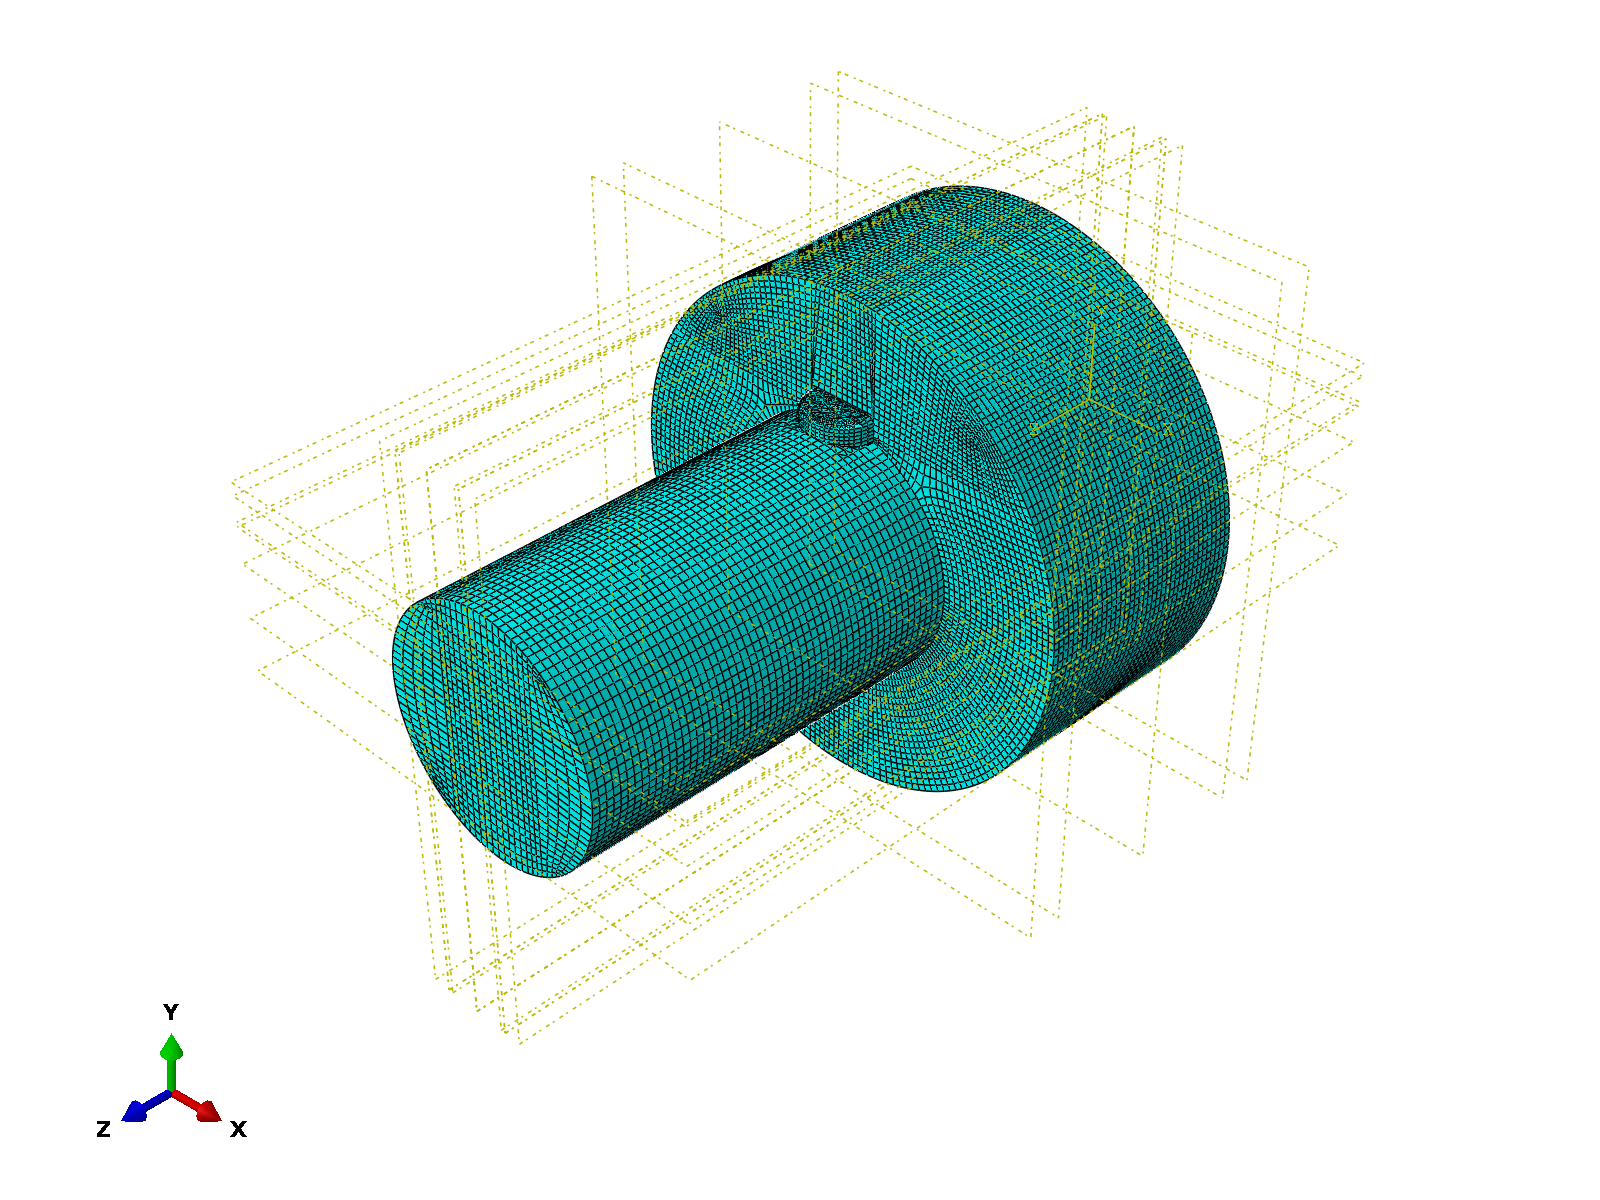
\includegraphics[width=\textwidth]{keyFormA-preview}\\[2pt]
  {\small (a) Form A -- rounded ends}
\end{minipage}\hfill
\begin{minipage}{0.48\textwidth}
  \centering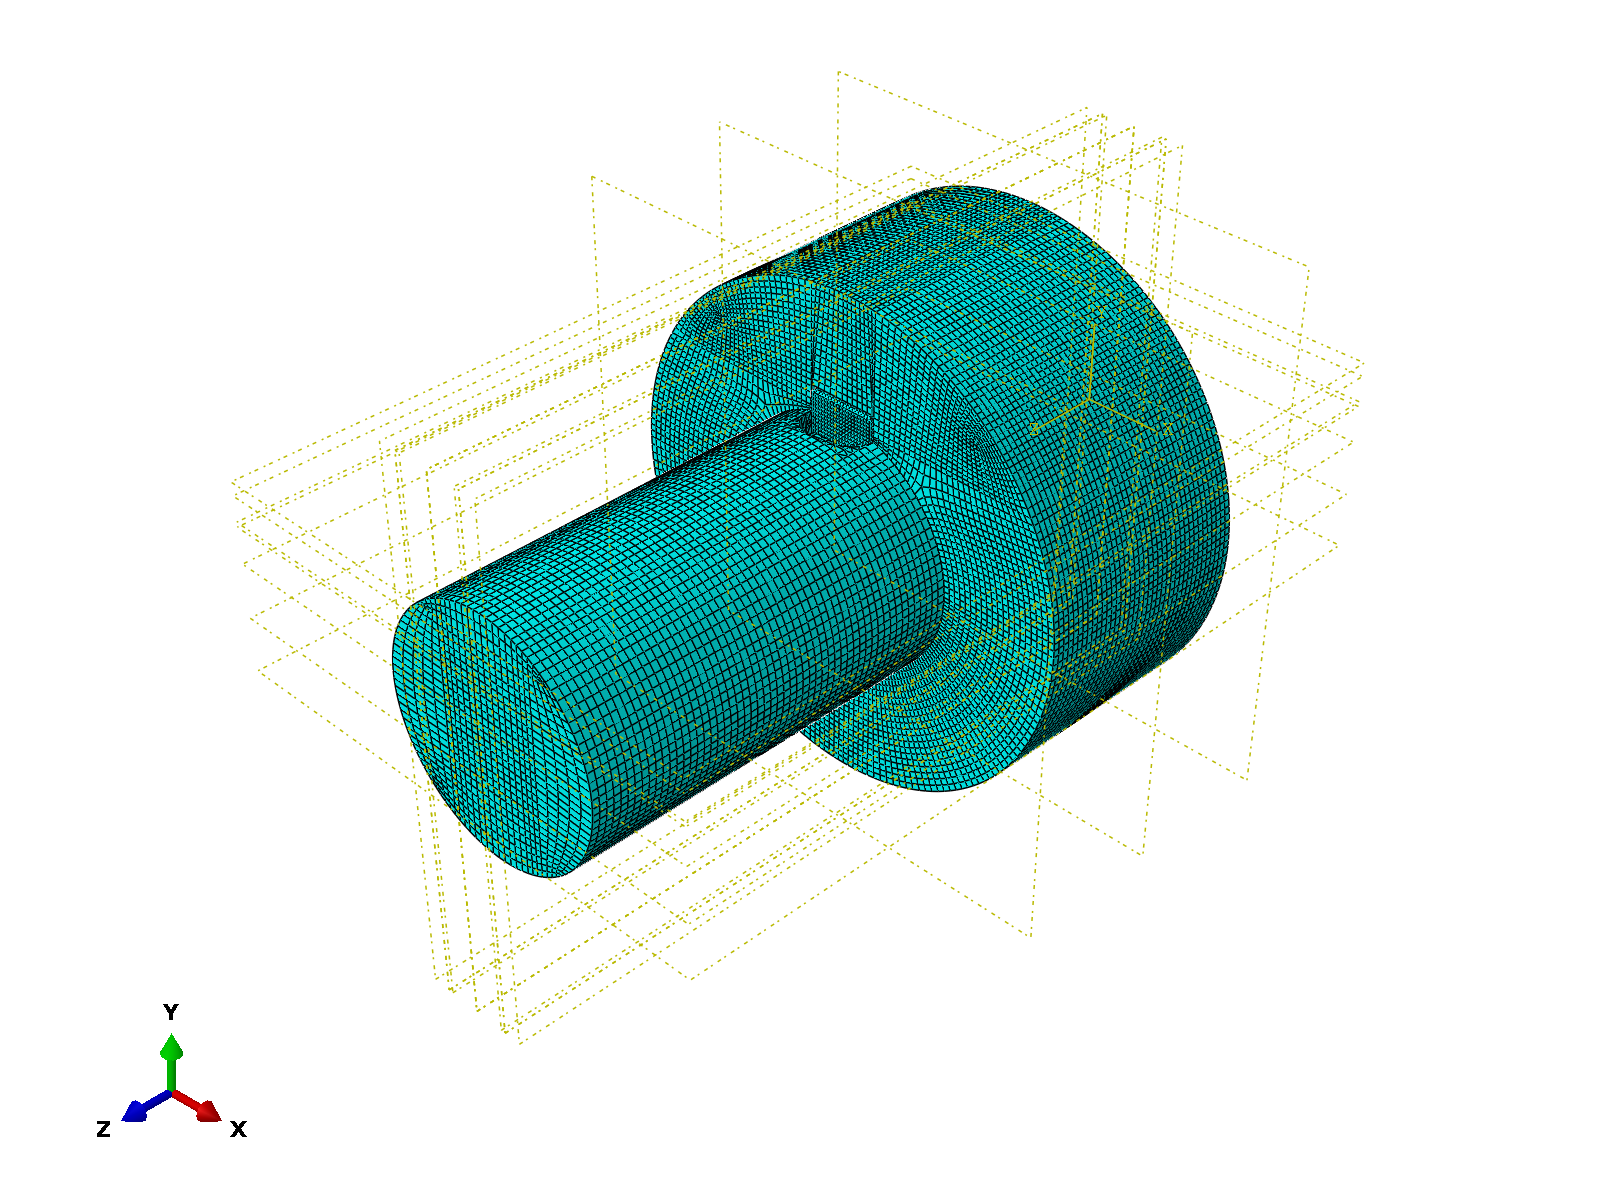
\includegraphics[width=\textwidth]{keyFormB-preview}\\[2pt]
  {\small (b) Form B -- square ends}
\end{minipage}
\caption{Meshed assembly for both key forms. The cylindrical hub is seated
directly on the shaft ($d_i = D$); no intermediate bushing is used.}
\label{fig:asm}
\end{figure}

% ==================================================================
\section{Materials and section assignments}
\label{sec:mat}
This section is deliberately split into the material definitions and the section
assignments, since the two are distinct objects in Abaqus.

\subsection{Materials}
Three materials are defined, one per component, all of grade \textbf{C45} steel
and all linear elastic:

\begin{center}
\begin{tabular}{llccc}
\toprule
Name & Grade & $E$ [MPa] & $\nu$ & $\rho$ [t/mm$^3$] \\
\midrule
\id{STEEL\_SHAFT} & C45 & $210\,000$ & $0.30$ & $7.85\times10^{-9}$ \\
\id{STEEL\_HUB}   & C45 & $210\,000$ & $0.30$ & $7.85\times10^{-9}$ \\
\id{STEEL\_KEY}   & C45 & $210\,000$ & $0.30$ & $7.85\times10^{-9}$ \\
\bottomrule
\end{tabular}
\end{center}

\noindent
A reference yield strength $R_e = 430\unit{MPa}$ is recorded for each material in
the audit file for later use. It is documentation only: no plastic law is
defined, so the present model is purely linear elastic.

\subsection{Sections and assignments}
Each component receives its \emph{own} homogeneous solid section, rather than
sharing one section between several parts:

\begin{center}
\begin{tabular}{lll}
\toprule
Section & Material & Assigned to \\
\midrule
\id{SEC\_STEEL\_SHAFT} & \id{STEEL\_SHAFT} & Shaft \\
\id{SEC\_STEEL\_HUB}   & \id{STEEL\_HUB}   & Hub \\
\id{SEC\_STEEL\_KEY}   & \id{STEEL\_KEY}   & Key \\
\bottomrule
\end{tabular}
\end{center}

\noindent
Separating them allows the grade of one component to be changed independently,
which is the usual case in practice (for example a harder key).

% ==================================================================
\section{Element choice and mesh strategy}
\label{sec:mesh}

\subsection{Element type: fully integrated}
The mesh uses \textbf{fully integrated} elements throughout. No reduced
integration is used anywhere in the model.

\begin{center}
\begin{tabular}{llll}
\toprule
Order & Hexahedron & Tetrahedron (fill) & Integration \\
\midrule
linear (default) & \id{C3D8} & \id{C3D4} & full \\
quadratic & \id{C3D20} & \id{C3D10} & full \\
\bottomrule
\end{tabular}
\end{center}

\noindent
A remark worth recording: the fully integrated \id{C3D8} is susceptible to shear
locking in bending, which stiffens the response. The element \id{C3D8I} is also
fully integrated but adds incompatible modes that remove this effect, and it is
available as an option. Neither \id{C3D8R}, \id{C3D20R} nor \id{C3D10M} is used,
as all three are reduced or modified formulations.

\subsection{Partitioning}
Each solid is divided into simpler cells so that it can be meshed with the
\id{STRUCTURED} technique where possible and \id{SWEEP} otherwise.

One partitioning detail deserves comment. In the shaft, the straight keyway wall
meets the semicircular cap \emph{tangentially} at the arc-centre planes. Cutting
there truncates a smooth ($G^1$) transition into a zero-angle cusp that no
hexahedron can fill. Cutting instead at the keyway extremes $z_0$ and $z_1$ was
measured to leave only two non-hexahedral cells out of $72$, against four when
cutting at the arc centres. The latter scheme is therefore used.

\subsection{Quality criteria and automatic repair}
After meshing, each part is audited for failed elements, warning elements,
aspect ratio, and connectivity (exactly one connected component per part). Cells
that still contain a failed element, or an element whose aspect ratio exceeds a
configurable threshold, are re-meshed with free tetrahedra. This guarantees
\emph{failed} $= 0$ while keeping the mesh predominantly hexahedral. The
threshold is a deliberate trade-off: raising it favours hexahedra, lowering it
favours a better worst-case aspect ratio.

% ==================================================================
\section{Parameter scheme}
\label{sec:param}
The parameters are split into those the user chooses and those the standard
fixes. This separation is what prevents an inconsistent key from being built.

\subsection{User parameters}
\begin{center}
\begin{tabular}{llll}
\toprule
Group & Parameter & Symbol & Default \\
\midrule
Shaft & diameter & $D$ & $40\unit{mm}$ \\
      & length ratio & $L/D$ & $3.0$ \\
      & arc-centre distance & $\Delta z$ & $38\unit{mm}$ \\
      & keyway start offset & --- & $5\unit{mm}$ \\
      & cap radius (0 = auto $b/2$) & $R_{\text{cap}}$ & auto \\
      & root fillet & $r_2$ & $0.25\unit{mm}$ \\
Key   & length (0 = auto) & $l$ & auto \\
      & corner chamfer & $c$ & $0.8\unit{mm}$ \\
      & chamfer angle & $\varphi_c$ & $45^\circ$ \\
Hub   & length & $L_{\text{hub}}$ & $38\unit{mm}$ \\
      & diameter ratio & $Q_A$ & $2.0$ \\
      & keyway roof fillet & $r_1$ & $0.25\unit{mm}$ \\
\bottomrule
\end{tabular}
\end{center}

\subsection{Derived parameters}
\begin{center}
\begin{tabular}{lll}
\toprule
Quantity & Relation & Value at $D=40$ \\
\midrule
Shaft radius & $R = D/2$ & $20.000$ \\
Shaft length & $L = 3D$ & $120.000$ \\
Key width & $b$ from DIN 6885 & $12.00$ \\
Key height & $h$ from DIN 6885 & $8.00$ \\
Shaft keyway depth & $t_1$ from DIN 6885 & $5.00$ \\
Hub keyway depth & $t_2$ from DIN 6885 & $3.30$ \\
Cap radius & $R_{\text{cap}} = b/2$ & $6.00$ \\
Keyway start & $z_0 = R_{\text{cap}} + 5$ & $11.00$ \\
Keyway end & $z_1 = z_0 + 2R_{\text{cap}} + \Delta z$ & $61.00$ \\
Keyway floor & $y_F = R - t_1$ & $15.000$ \\
Key base & $y_{\min} = R - t_1$ & $15.000$ \\
Key top & $y_{\max} = R - t_1 + h$ & $23.000$ \\
Key half width & $x_w = b/2$ & $6.00$ \\
Hub bore & $d_i = D$ & $40.00$ \\
Hub outer & $d_a = D\,Q_A$ & $80.00$ \\
Hub keyway roof & $R + t_2$ & $23.300$ \\
Top clearance & $g_c = t_1 + t_2 - h$ & $0.300$ \\
\bottomrule
\end{tabular}
\end{center}

\subsection{Justification of the corner chamfer \texorpdfstring{$c$}{c}}
\label{sec:cham}
The chamfer size is not arbitrary. The lower corner chamfer of the key must
clear the \emph{root fillet} $r_2$ of the shaft keyway. The fillet centre lies at
$(x_w - r_2,\; y_F + r_2)$, and both of its tangent points satisfy
\begin{equation}
y - x = y_F - x_w + r_2 ,
\end{equation}
while the chamfer face is the line
\begin{equation}
y - x = y_{\min} - (x_w - c) .
\end{equation}
Since $y_{\min} = y_F$, the requirement collapses to the compact condition
\begin{equation}
\boxed{\;c \ge r_2\;}
\qquad\text{with}\qquad
\text{clearance} = \frac{c - r_2}{\sqrt{2}} .
\label{eq:cham}
\end{equation}
For the nominal design ($r_2 = 0.25$, $c = 0.8$) this gives a perpendicular
clearance of $0.3889\unit{mm}$, and the upper chamfer keeps $0.6086\unit{mm}$
from the hub roof fillet $r_1$. Both values are computed and printed by the
builder, so the choice $c = 0.8\unit{mm}$ is justified rather than assumed. Two
further consequences are reported: the straight flank height left to carry
torque, $h - 2c = 6.400\unit{mm}$, and the hub wall remaining above its keyway,
$d_a/2 - (R + t_2) = 16.700\unit{mm}$.

Equation~\eqref{eq:cham} was verified numerically: setting $c = 0.20$, below
$r_2$, makes the builder report a clearance of $-0.0354\unit{mm}$ and the overall
verdict changes to CHECK.

% ==================================================================
\section{Verification results}
\label{sec:results}
Both key forms were built at the nominal diameter $D = 40\unit{mm}$ with mesh
seeds of $1.2$, $0.6$ and $1.0\unit{mm}$ for shaft, key and hub. Element codes
are \id{C3D8} (hexahedra) and \id{C3D4} (tetrahedral fill).

\begin{table}[H]
\centering
\caption{Mesh statistics, Form A key (rounded ends).}
\begin{tabular}{lrrrrrr}
\toprule
Part & Nodes & Elements & \id{C3D8} & \id{C3D4} & AR worst & AR avg \\
\midrule
Shaft & $86\,341$ & $80\,515$ & $79\,175$ & $1\,340$ & $21.32$ & $1.425$ \\
Key   & $31\,101$ & $31\,873$ & $27\,120$ & $4\,753$ & $6.32$ & $1.803$ \\
Hub   & $161\,265$ & $149\,720$ & $149\,720$ & $0$ & $5.40$ & $1.283$ \\
\midrule
\textbf{Total} & $278\,707$ & $262\,108$ & $256\,015$ & $6\,093$ & --- & --- \\
\bottomrule
\end{tabular}
\end{table}

\begin{table}[H]
\centering
\caption{Mesh statistics, Form B key (square ends).}
\begin{tabular}{lrrrrrr}
\toprule
Part & Nodes & Elements & \id{C3D8} & \id{C3D4} & AR worst & AR avg \\
\midrule
Shaft & $86\,341$ & $80\,515$ & $79\,175$ & $1\,340$ & $21.32$ & $1.425$ \\
Key   & $22\,680$ & $20\,212$ & $20\,212$ & $0$ & $3.25$ & $1.248$ \\
Hub   & $161\,265$ & $149\,720$ & $149\,720$ & $0$ & $5.40$ & $1.283$ \\
\midrule
\textbf{Total} & $270\,286$ & $250\,447$ & $249\,107$ & $1\,340$ & --- & --- \\
\bottomrule
\end{tabular}
\end{table}

\noindent
The hexahedral fraction is $97.7\,\%$ for Form A and $99.5\,\%$ for Form B. In
both cases every part has \emph{failed} $= 0$ and exactly one connected
component. The Form B key is entirely hexahedral. The remaining tetrahedra sit
in the rounded caps of the keyway and, for Form A, of the key: there the straight
wall meets the cap arc tangentially, which no hexahedron can fill.

\subsection{Fit and clearance checks}
All checks are evaluated analytically from the parameters and reported with a
pass or fail flag:

\begin{center}
\begin{tabular}{lcl}
\toprule
Check & Value [mm] & Status \\
\midrule
Shaft OD vs hub bore & $0.0000$ & line-to-line seat \\
Key base vs keyway floor & $0.0000$ & seated \\
Shaft keyway flank per side & $0.0000$ & line-to-line \\
Hub keyway flank per side & $0.0107$ & clearance \\
Key top vs hub roof, $g_c$ & $0.3000$ & clearance \\
Key length vs keyway & $0.0000$ & at the limit \\
Chamfer $c$ vs root fillet $r_2$ & $0.5500$ & $c \ge r_2$ satisfied \\
Bottom chamfer clearance & $0.3889$ & clear \\
Top chamfer clearance & $0.6086$ & clear \\
Straight flank left, $h-2c$ & $6.4000$ & load-carrying \\
Hub wall left above keyway & $16.7000$ & no breakthrough \\
\bottomrule
\end{tabular}
\end{center}

\subsection{Behaviour away from the nominal size}
The scheme was also verified at $D = 50\unit{mm}$. DIN 6885 switches the key to
$b = 14$, $h = 9$, $t_1 = 5.5$, $t_2 = 3.8$, and the derived quantities follow:
$R = 25$, $L = 150$, $R_{\text{cap}} = 7$, $z_0 = 12$, $z_1 = 64$,
$y_F = 19.5$, $d_a = 100$, roof $= 28.8$ and again $g_c = 0.300$. The build
completes with verdict OK and a hexahedral fraction of $97.9\,\%$.

% ==================================================================
\section{Response to the review comments}
\label{sec:review}
\begin{center}
\begin{tabular}{p{0.30\textwidth}p{0.62\textwidth}}
\toprule
\textbf{Comment} & \textbf{Action taken} \\
\midrule
Sec.~3 -- why a tapered hub? &
The tapered bushing was removed from the default configuration. The hub is now
cylindrical and seated directly on the shaft, $d_i = D$, consistent with the
parameter scheme. See Section~\ref{sec:geom}. \\
\addlinespace
Sec.~4 -- please divide sections &
Section~\ref{sec:mat} is now split into material definitions and section
assignments. In the model itself, each part carries its own section
(\id{SEC\_STEEL\_SHAFT}, \id{SEC\_STEEL\_HUB}, \id{SEC\_STEEL\_KEY}) instead of
sharing one. \\
\addlinespace
\id{C45QT\_KEY} $\rightarrow$ \id{steel\_key}; also \id{STEEL\_SHAFT},
\id{STEEL\_HUB} &
Materials renamed to \id{STEEL\_SHAFT}, \id{STEEL\_HUB} and \id{STEEL\_KEY},
all of grade C45. \\
\addlinespace
Sec.~5 -- rely on linear hexahedral elements, fully integrated &
Default is \id{C3D8} with \id{C3D4} fill; the quadratic option is \id{C3D20}
with \id{C3D10}. No reduced-integration element remains. Hexahedral fraction
$97.7$--$99.5\,\%$. See Section~\ref{sec:mesh}. \\
\addlinespace
Sec.~6.1 -- why $c = 0.8$? &
Derived, not assumed: the chamfer must clear the root fillet, giving
$c \ge r_2$ and a clearance $(c-r_2)/\sqrt{2}$. See
Section~\ref{sec:cham} and Eq.~\eqref{eq:cham}. \\
\addlinespace
Key $\rightarrow$ switch Form A / Form B &
Implemented as a switch. Form A has rounded ends, Form B square ends; the
admissible length differs and is checked. See Section~\ref{sec:key}. \\
\addlinespace
$b$, $h$ dependent on $D$ (DIN 6885) &
Read from the DIN 6885-1 table; not editable by hand. \\
\addlinespace
Hub: $L_{\text{hub}}$, $d_i = D$, $Q_A$, $d_a = D\,Q_A$, $r_1$,
$g_c = t_1 + t_2$ &
All implemented as given; $g_c$ follows Eq.~\eqref{eq:gc}. \\
\bottomrule
\end{tabular}
\end{center}

% ==================================================================
\section{Scope and limitations}
\begin{enumerate}\itemsep3pt
  \item The model is in the \textbf{NOJOB} state. It contains geometry,
        materials, mesh, assembly and sets, and only the \id{Initial} step. No
        contact, analysis step, boundary condition, load or job is defined, so it
        can be inspected but not yet submitted to the solver.
  \item The material response is linear elastic. The reference yield strength is
        recorded but no plastic law is defined; no statement about yielding can
        be made from this model.
  \item The worst aspect ratio, about $21$, occurs next to the $r_2 = 0.25$
        root fillet of the shaft, where a small radius meets a much coarser
        surrounding mesh. It is a mesh-quality figure, not a result.
  \item A small number of tetrahedra remain in the rounded cap regions for the
        geometric reason given in Section~\ref{sec:results}. Their count is
        reported per part in the audit file.
  \item The fillet $r_1$ is interpreted as the fillet at the roof corners of the
        hub keyway, mirroring $r_2$ in the shaft. If a different feature was
        intended, this should be confirmed.
\end{enumerate}

\vfill
\noindent\footnotesize
Prepared by [Your name]. All numerical values in this report were produced by the
parametric builder and taken from its audit output.

\end{document}
